%-----------------------------------------------------------------------
% SCIENCE CHINA Information Sciences -- Research Paper
% Template: SCIS2026.cls (official, downloaded from scis.scichina.com)
%-----------------------------------------------------------------------
\documentclass{SCIS2026}

%%%%%%%%%%%%%%%%%%%%%%%%%%%%%%%%%%%%%%%%%%%%%%%%%%%%%%%
%%% Author's definitions for this manuscript
%%%%%%%%%%%%%%%%%%%%%%%%%%%%%%%%%%%%%%%%%%%%%%%%%%%%%%%
\graphicspath{{figs/}}
%% generated by mkart_scis.py -- do not edit
\newcommand{\nProbs}{15}
\newcommand{\budget}{10^{5}}
\newcommand{\seeds}{30}
\newcommand{\seedsExt}{20}
\newcommand{\refFrontPts}{400}
\newcommand{\nProbedDirect}{39}
\newcommand{\nGridCells}{81}
\newcommand{\retMthree}{91}
\newcommand{\retMfive}{85}
\newcommand{\retMeight}{72}
\newcommand{\retMten}{65}
\newcommand{\retMthreeDef}{9}
\newcommand{\retMfiveDef}{15}
\newcommand{\retMeightDef}{28}
\newcommand{\retMtenDef}{35}
\newcommand{\retWorst}{45}
\newcommand{\retWorstWhere}{200,10}
\newcommand{\retWorstAll}{75}
\newcommand{\retExactFrac}{8.7}
\newcommand{\retCombos}{13895}
\newcommand{\retExceed}{0}
\newcommand{\nFilesTotal}{1887}
\newcommand{\nFilesAffected}{84}
\newcommand{\pctAffected}{4.5}
\newcommand{\nAlgTotal}{360}
\newcommand{\nAlgAffected}{83}
\newcommand{\pctAlgAffected}{23.1}
\newcommand{\nAlgSingle}{82}
\newcommand{\nCommentHits}{0}
\newcommand{\nReuseZ}{42}
\newcommand{\fixMaxGain}{11.1}
\newcommand{\fixMinGain}{-4.1}
\newcommand{\fixMedGain}{1.7}
\newcommand{\fixNoWorseN}{13}
\newcommand{\fixWorseN}{2}
\newcommand{\fixTinyN}{1}
\newcommand{\fixSigCount}{4}
\newcommand{\fixSigHolm}{1}
\newcommand{\cliffMax}{0.64}
\newcommand{\ciExclN}{8}
\newcommand{\layerN}{15}
\newcommand{\layerMedHost}{+0.87}
\newcommand{\layerMedMatched}{+0.04}
\newcommand{\layerBetterHost}{10}
\newcommand{\layerWorseHost}{5}
\newcommand{\layerBetterMatched}{8}
\newcommand{\layerWorseMatched}{7}
\newcommand{\layerBigN}{6}
\newcommand{\layerShrinkMin}{0.9}
\newcommand{\layerShrinkMax}{8.8}
\newcommand{\layerSmallMax}{8.6}
\newcommand{\layerBeatsStaticN}{2}
\newcommand{\layerStrongN}{6}
\newcommand{\layerStrongBeatsN}{2}
\newcommand{\genHost}{552}
\newcommand{\genFix}{499}
\newcommand{\genRatio}{1.106}
\newcommand{\popRatio}{1.099}
\newcommand{\feHost}{100090}
\newcommand{\feFix}{100000}
\newcommand{\feOver}{90}
\newcommand{\feOverPct}{0.09}
\newcommand{\angRatioThree}{1.45}
\newcommand{\angNbiThree}{5.19}
\newcommand{\angMudThree}{3.57}
\newcommand{\angNbiFive}{18.19}
\newcommand{\angMudFive}{7.89}
\newcommand{\angRatioFive}{2.31}

%% generated by mkart_audit.py -- do not edit
\newcommand{\nTraced}{16}
\newcommand{\nTracedAff}{13}
\newcommand{\nTracedCtl}{3}
\newcommand{\nRealMin}{31}
\newcommand{\nRealMinAlg}{RVEAa}
\newcommand{\ctlNames}{NSGAII, SPEA2, IBEA}
\newcommand{\nLexFiles}{84}
\newcommand{\nLexBefore}{62}
\newcommand{\nLexAfter}{6}
\newcommand{\nLexNoInit}{16}
\newcommand{\nLexReuseZ}{42}
\newcommand{\pctLexBefore}{74}
\newcommand{\nAlgFaithful}{277}

%% generated by xplatform.py -- do not edit
\newcommand{\nPlatMthree}{91}
\newcommand{\nPlatMfive}{85}
\newcommand{\nPlatMeight}{72}
\newcommand{\nPlatMten}{65}
\newcommand{\nPymoMeight}{36}
\newcommand{\xRatioEight}{2.00}
\newcommand{\nPymoMfive}{70}
\newcommand{\xRatioFive}{1.21}
\newcommand{\nXDiverging}{3}
\newcommand{\nXCases}{5}

%% generated by mkart_round13.py -- do not edit
\newcommand{\nAbcProblems}{15}
\newcommand{\abcDeclVsPubAbsMed}{1.2}
\newcommand{\abcDeclVsPubSignedMed}{+0.0}
\newcommand{\abcDeclVsPubMax}{4.2}
\newcommand{\abcRepVsDeclMed}{2.7}
\newcommand{\abcRepVsDeclPos}{11}
\newcommand{\abcRepVsDeclTie}{1}
\newcommand{\abcRepVsDeclNeg}{3}
\newcommand{\abcRepVsPubMed}{+1.7}
\newcommand{\abcRepVsPubPos}{12}
\newcommand{\abcRepVsPubTie}{1}
\newcommand{\abcRepVsPubNeg}{2}
\newcommand{\abcPairs}{15}
\newcommand{\abcIndistinct}{15}
\newcommand{\abcMinP}{0.12}
\newcommand{\abcDeclReqMthree}{91}
\newcommand{\abcDeclReqMfive}{85}
\newcommand{\kProblems}{15}
\newcommand{\kWinsThree}{5}
\newcommand{\kWinsFive}{3}
\newcommand{\kWinsTen}{7}
\newcommand{\kSpreadMed}{9.6}
\newcommand{\kFailRatio}{26723}
\newcommand{\kFailProblem}{DTLZ1}
\newcommand{\kFailK}{10}
\newcommand{\kFailValue}{1116.0}
\newcommand{\kFailBest}{0.0418}
\newcommand{\kFailBadSeeds}{29}
\newcommand{\kFailN}{1}


\begin{document}
%\oa

\ArticleType{RESEARCH PAPER}
\Year{2026}
\Month{October}
\Vol{69}
\No{1}
\DOI{}
\ArtNo{}
\ReceiveDate{}
\ReviseDate{}
\AcceptDate{}
\OnlineDate{}
\AuthorMark{Zhang Y X}
\AuthorCitation{Zhang Y X}

\title{A population-size fidelity framework for reference-vector multi-objective evolutionary algorithms with an audit of PlatEMO}{A population-size fidelity framework for reference-vector MOEAs}

\author[1]{Yuxuan ZHANG}{{Zhangyuxuan@aeu.edu.cn}}

\address[1]{Graduate School, Army Engineering University of PLA, Nanjing 210007, China}

\abstract{Reference-vector multi-objective evolutionary algorithms derive their population from a reference-vector constructor, and a comparison is credible only if the used size is the reported size. We show that in PlatEMO 4.16 this can fail silently, and turn it into a reusable audit. The framework separates three quantities, requested, evaluated, recorded, and provides a fidelity principle with two propositions, an audit, a repair catalogue and a reporting protocol. The lexical audit finds the assignment in 84 of 1887 files, belonging to 83 of the platform's 360 algorithms. A trace of sixteen algorithms shows the consequence: configuring 100 realises 91 individuals for nine of the thirteen affected algorithms, as few as 31 for the four that shrink their reference set, and 100 for three unaffected ones, so a table reporting 100 throughout compares populations differing by more than a factor of three. The platform records the constructor's cardinality rather than the request, without flagging the divergence. On a fifteen-problem suite, restoring the requested size improves the median indicator on twelve problems, barely on a thirteenth and not on two, and reduces the layer's median gain from \layerMedHost\% to \layerMedMatched\%; three repair cases occur in practice, so no repair is universal.}

\keywords{population-size fidelity, reference-vector algorithm, benchmarking reproducibility, evolutionary multi-objective optimization, PlatEMO, fair comparison, large-scale optimization}

\maketitle

%%%%%%%%%%%%%%%%%%%%%%%%%%%%%%%%%%%%%%%%%%%%%%%%%%%%%%%
%%% The main text
%%%%%%%%%%%%%%%%%%%%%%%%%%%%%%%%%%%%%%%%%%%%%%%%%%%%%%%

\section{Introduction}
Decomposition-based and reference-vector multi-objective evolutionary algorithms (MOEAs) dominate current practice, and their population is organised around a set of reference vectors whose cardinality is taken to be the population size $N$~\cite{1,2,3}. The field is moving quickly on two fronts at once. Large language models are being woven into the evolutionary loop as offspring generators, operator designers and hyper-heuristics, and the first surveys of this intersection have appeared~\cite{4,5,6}. In parallel, large-scale and many-objective problems keep raising what a reference-vector method must deliver, as the most recent surveys of large-scale multi-objective optimization make clear~\cite{7,8}. Across both fronts one quantity is quietly load-bearing: the population size. It fixes the number of reference vectors and therefore the resolution of the search, it fixes the evaluation budget consumed per generation and therefore how many generations fit into a fixed budget, and it is reported in every experimental section as a controlled quantity. Whether a comparison is fair hinges on it, a point made explicitly in recent community guidance on fair benchmarking of evolutionary multi-objective algorithms, which names the population size among the few experimental choices that most distort a comparison~\cite{9,10}.

We report that in a widely used platform this controlled quantity is not, in general, what it appears to be, and we argue that the underlying failure mode is general enough to deserve a framework. In PlatEMO~\cite{11}, a reference-vector set is obtained by calling a constructor that returns both the vectors and their number. A large number of algorithm files pass the user's population size to that constructor and then assign the second output back to the population size, so that the requested size is silently replaced by the size of the reference lattice. The constructor does not return the requested size: over the range $2\le M\le 15$, $M\le N\le 1000$, it never returns more points than requested and returns exactly the requested number in only \retExactFrac\% of cases. At $N=100$ the platform therefore runs with \retMthree{} individuals at three objectives and \retMten{} at ten objectives, a reduction of \retMthreeDef\% and \retMtenDef\% with no message to the user. The same mechanism can be present in any library that returns a reference set together with a size that is then written into a shared problem object.

Three quantities have to be kept apart, because the whole failure lives in the gap between them: the size a study requests and declares, $N_{\mathrm{req}}$; the size the method actually evaluates, $N_{\mathrm{real}}$; and the size the run records, $N_{\mathrm{rep}}$. We traced all three in the platform studied here (Table~\ref{tab:trace}), and the outcome is unambiguous: the constructor returns 91 for a request of 100, and nine of the thirteen affected algorithms then evaluate exactly those 91 individuals, so for those nine $N_{\mathrm{real}} = N_{\mathrm{rep}} = \retMthree{}$ while $N_{\mathrm{req}} = 100$; the other four evaluate fewer. The platform always records the constructor's cardinality --- never the request, which the assignment has overwritten --- so for the four algorithms that shrink their own reference set during the search it does not record the size actually used either, and the recorded figure overstates the population. What is missing throughout is any signal that the request was not honoured, and the consequence is a confounded comparison rather than a corrupted result. In the same release, NSGA-II, SPEA2 and IBEA contain no such assignment and run at exactly 100, so a table that reports $N=100$ while mixing NSGA-III with NSGA-II, or MOEA/D with SPEA2, or RVEA with IBEA, is comparing 91, 83, 80, 66 or 31 with 100. The nominal size in the table is the same; the runs are not.

That is the failure the framework addresses, and it is a reporting failure rather than a coding mistake. The rounding itself is unavoidable: a symmetric lattice in $M$ objectives admits only certain cardinalities, so a request that falls between two admissible values has to be rounded. What is avoidable is that the rounded value replaces the requested one without the study being told, so that the number printed in the experimental section is no longer the number the run used. It follows that the remedy is not to forbid the write-back, which many algorithms use deliberately to keep the population and the reference set consistent, but to make the divergence visible and to report the size that was realised.

The size actually realised leaves traces that a reader can check without instrumenting the platform, which is what makes the problem detectable rather than merely suspected. The per-generation cost of a reference-vector method is proportional to $N_{\mathrm{real}}$, so under a fixed evaluation budget the number of completed generations is inversely proportional to it; in our controlled runs the declared size of 100 corresponds to \genFix{} generations and the realised size of 91 to \genHost{}, a ratio of \genRatio{} against the predicted \popRatio{}. A study that reports its generation count, or publishes convergence curves against generations, therefore exposes the discrepancy, and a study that reports only the final indicator hides it.

The mechanism is easy to miss, and we missed it ourselves: it surfaced only when a controlled comparison of an adaptive scheduling layer refused to reproduce. An earlier version of that layer appeared to improve its host algorithm by a double-digit percentage, and the improvement survived visual inspection of convergence curves. It did not survive matching the population size, because the host was running with 91 individuals while the layer ran with 100.

We therefore present the episode not as a bug report but as the framework for \emph{population-size fidelity} that it motivates: the property that the population size a method runs with equals the size it reports. The framework has four parts. First, a fidelity principle that states what must hold and why a violation is a threat to reproducible comparison, since reproducibility in evolutionary computation is itself an established concern~\cite{12}. Second, an auditing procedure that locates the offending constructor calls in a code base. Third, a catalogue of corrections, which shows that a single one-line repair is not universally valid and that the admissible repair depends on how an algorithm couples its population to its reference set. Fourth, a reporting protocol that makes violations visible in future work. We then apply the whole framework to PlatEMO 4.16 as a case study, quantify the consequences with controlled experiments on a large-scale suite, and show that the framework is what turns an isolated observation into a checkable, reusable procedure.

The contribution is therefore not the disclosure of a defect but the construction and validation of an instrument. Specifically, the paper (i) separates the requested, realised and reported sizes and formalises fidelity over them, proving that the deficit introduced by a lattice constructor is one-signed and inflates the number of generations completed under a fixed budget; (ii) reduces the search for infidelity to an auditable pattern, tested against fourteen positive and negative cases; (iii) shows by construction that the repair is algorithm-dependent, with three cases realised by real algorithms and the mechanism of the hardest case measured rather than asserted; (iv) quantifies the consequences on a fifteen-problem suite with a paired design, effect sizes and a three-arm control that separates the two effects a single comparison conflates; and (v) supplies a reporting protocol together with fully released materials.

\section{Related work}
\label{sec:related}
Four strands of recent work frame this study. The first is the reference-vector family itself. Reference-vector guided selection remains the workhorse for many-objective problems, and recent methods continue to build on it, for example by adapting the reference vectors to sparse or irregular fronts and by replacing the convergence measure used inside selection~\cite{13}. In all of these methods the population size is the hidden constant, because the reference set and the population are indexed by the same $N$.

The second strand is the benchmarking-methodology literature. Community guidance has long warned that an indicator value is comparable only when the experimental protocol is fixed~\cite{14,15}, and comparison results have since been shown to depend strongly on the specification of the population size, the quantity we audit~\cite{9}; wall-clock time rather than evaluations alone has been argued to be the budget that matters in practice~\cite{16}; the reproducibility of evolutionary computation has been examined in its own right~\cite{12}; the rigour of the field has been critically reviewed~\cite{17}; and the design of benchmarks with practical impact has been reconsidered~\cite{18}. The closest antecedent to our work is an analysis of single-objective algorithms implemented across thirteen frameworks, which found that even identical parameter settings can yield different results because of implementation differences; that study raises the general concern and calls for guidelines, but it does not isolate a mechanism that a reader can check, and it covers single-objective algorithms~\cite{10}. Our contribution is a mechanism of exactly that kind, located in the reference-vector constructor, together with the audit and the repairs that make it actionable.

The third strand is the rapid arrival of methods driven by large language models, which generate offspring, design operators and steer multi-objective search end to end~\cite{4,5,6,19}, and are almost always benchmarked against reference-vector baselines drawn from the same platforms that we audit. A systematic population-size mismatch in those baselines would therefore propagate into the comparisons that this fast-moving literature uses to establish its gains.

The fourth strand is the widening of the problem classes to which reference-vector methods are applied: surrogate-assisted methods for expensive and high-dimensional problems, and constrained variants, are surveyed at increasing frequency~\cite{20,21,22}, and every one of these families inherits the reference-vector selection machinery and, with it, the population-size convention under audit. The fidelity problem is therefore not tied to one benchmark but to the shared substrate of a whole class of methods.

\section{The population-size fidelity framework}
\label{sec:framework}
We now state the framework in a form that is independent of any particular library. Throughout, a \emph{reference-vector method} is an algorithm whose population is organised around a finite set of reference vectors, the symbol $N$ denotes the population size that the user sets, and $M$ denotes the number of objectives.

\subsection{The fidelity principle}
\label{sec:principle}
We first make the notion precise, because the whole framework rests on distinguishing three quantities that are usually conflated.

\begin{definition}[Population-size fidelity]
Consider a reference-vector method configured with a requested size $N_{\mathrm{req}}$, evaluating a population $P$ of size $N_{\mathrm{real}} = |P|$, and recording a size $N_{\mathrm{rep}}$ in its own output. The method is \emph{population-size faithful} if $N_{\mathrm{req}} = N_{\mathrm{real}} = N_{\mathrm{rep}}$. Otherwise it suffers a \emph{size infidelity}, and we call $\delta = N_{\mathrm{req}} - N_{\mathrm{real}}$ its \emph{size drift}.
\end{definition}

The definition isolates the three quantities deliberately, because a run can satisfy any two while violating the third. Three variants of the failure are worth separating. A run that rounds its request and then records the rounded value is honest about what it did: it is unfaithful only in the sense that the request could not be honoured, and the discrepancy is found by comparing $N_{\mathrm{req}}$ with $N_{\mathrm{real}}$ before the run rather than after it. A run that rounds, records the rounded value faithfully, and is then written up in a study whose tables state the original request is the case that threatens a comparison; there the platform is right and the paper is not, and the discrepancy is found by comparing the number in the table with the number the run realised. A run whose population changes again after the constructor has returned --- because the algorithm prunes its own reference set --- leaves a record that matches neither the request nor the population, and then the platform itself overstates the run. Section~\ref{sec:case} shows that PlatEMO produces the second variant for all affected algorithms and the third variant as well for four of them. All three quantities are observable without modifying the method or the library: $N_{\mathrm{req}}$ is what the study configures, $N_{\mathrm{real}}$ follows from the cardinality of the reference set and the evaluation cost of a generation, and $N_{\mathrm{rep}}$ is what the run stores. This is why an audit can rest on the definition rather than on the intent of the code.

Fidelity matters for three reasons. First, the realised population fixes the cardinality of the reference set and hence the resolution of the search. Second, it fixes the evaluation budget consumed per generation and therefore the number of generations that fit into a fixed budget. Third, the reported size is the quantity a reader uses to judge whether two methods were compared under the same conditions, and this third reason is the most insidious, because an unfaithful run still produces a valid Pareto approximation and raises no error.

It is useful to separate fidelity from quality: an unfaithful run is not necessarily a poor run, and a faithful run is not necessarily a good one. Fidelity is the weaker property that the experiment is what it claims to be --- exactly the property that a comparison across methods presupposes. It follows that restoring fidelity does not in itself improve an algorithm: it changes what the reported number means. The empirical sections below are written with this distinction in view, and we therefore report the direction and the size of every difference rather than treating fidelity as a performance claim.

The definition's practical interest comes from two facts that convert an anecdote into a checkable statement.

\begin{proposition}[Monotone downward drift]
Let $L(N,M)$ denote the number of rows of the matrix returned by the two-layer lattice constructor used in this study (Section~\ref{sec:case}) for a requested size $N$ and $M$ objectives; this is the cardinality the calling algorithm sees, and the size it writes back into the population field. Then $L(N,M) \le N$ for all $M \ge 2$, $N \ge M$, with equality if and only if $N$ is an admissible lattice size; consequently $\delta \ge 0$: the drift can only remove individuals, never add them.
\end{proposition}

\proof The constructor builds a first layer from the integer $H_1$, the smallest value with $\binom{H_1+M}{M-1}>N$. Because $H_1-1$ fails that inequality, $\binom{(H_1-1)+M}{M-1}\le N$, and the first layer contains exactly $\binom{H_1+M-1}{M-1} = \binom{(H_1-1)+M}{M-1}\le N$ rows; when $H_1=1$ the layer contains $\binom{M}{M-1}=M\le N$ rows, the boundary case being $M=N$. A second layer is added only if $H_1<M$ and the first layer is short of $N$; its size $H_2\ge 1$ is the smallest integer with $\binom{H_1+M-1}{M-1}+\binom{H_2+M}{M-1}>N$. Hence $H_2-1$ satisfies the opposite inequality, and the second layer actually contributes $\binom{H_2+M-1}{M-1}$ rows, exactly the binomial coefficient that the stopping condition bounds by $N-\binom{H_1+M-1}{M-1}$. The total is therefore at most $N$ and never exceeds the request. Equality requires that the stopping condition be met at the step that exhausts the request, that is, that $N$ coincide with an admissible lattice size; otherwise the constructor returns the largest admissible size below $N$. A duplicated row between the two layers would reduce the number of distinct directions but not the row count that $L(N,M)$ measures, so it cannot affect the inequality; we verified that no duplicate occurs over the tested range.

We verified the proposition exhaustively rather than trusting the argument alone. Over $2\le M\le 15$ and $M\le N\le 1000$, that is \retCombos{} distinct combinations, the realised count exceeds the request in \retExceed{} cases, and the two layers never yield a duplicated direction. The counts were also checked against the platform's own constructor at \nProbedDirect{} points spanning the range and at all \nGridCells{} cells of the grid reported in Table~\ref{tab:deficit}, with no disagreement.

The range is the range we scanned, not a documented limit: the platform's problems take the number of objectives as an argument, and its sources carry defaults up to ten (for example, the MaF8 problem declares \texttt{obj.M~=~10} as its default). The scan extends to $M=15$, half as much again beyond that default ceiling, which comfortably brackets the objective counts at which reference-vector methods are actually run and is cheap enough to enumerate completely; beyond it the closed form still applies at negligible cost. The complete table $L(N,M)$ over that range is released as a machine-readable file, and points outside it follow from the closed form of the constructor rather than from a measurement.

\begin{proposition}[Generation inflation]
Consider a method whose report and printed tables state a size $N_{\mathrm{req}}=N$, but which evaluates a population of size $N_{\mathrm{real}}=L<N$ and consumes $cL$ evaluations per generation for a constant $c>0$ fixed by the method, stopping when the evaluation budget $\mathrm{FE}_{\max}$ is exhausted. Then it completes $\lfloor \mathrm{FE}_{\max}/(cL) \rfloor$ generations where the reported size implies $\lfloor \mathrm{FE}_{\max}/(cN) \rfloor$, a relative excess of $(N-L)/L$ in the number of generations.
\end{proposition}

\proof The number of generations is the budget divided by the cost of a generation, which is $cN_{\mathrm{real}}$. Substituting $N_{\mathrm{real}}=L$ for the actual run and $N_{\mathrm{req}}=N$ for the reported condition, and taking the ratio, gives $N/L$, that is, an excess of $(N-L)/L$.

The premise of Proposition~2 is the reporting condition and not the internal mechanics: the excess appears whenever the quantity a study states is $N_{\mathrm{req}}$ while the quantity the run realises is $L$. A run that both realises $L$ and reports $L$ is described by the same formula with $N=L$ and shows no excess, which is the consistency condition of the framework. Two consequences follow. When the constructor is the one of Section~\ref{sec:case}, Proposition~1 makes the drift one-signed, so an unfaithful method is biased in a fixed direction rather than randomly perturbed. When the comparison is made under a fixed evaluation budget, Proposition~2 makes the drift translate directly into a difference in the number of generations, which is exactly the quantity that a convergence curve displays. Neither fact is visible from a single reported population size, which is why the framework is needed.

\subsection{Auditing a library for size infidelity}
\label{sec:audit-proc}
The audit rests on a single observation: size infidelity arises when the output of a reference-vector constructor is written into a shared object that stores the population size. Algorithm~\ref{alg:audit} formalises the procedure.

\begin{algorithm}
\footnotesize
%\floatname{algorithm}{Algorithm}
\caption{Auditing a library for population-size infidelity}
\label{alg:audit}
\begin{algorithmic}[1]
    \REQUIRE source tree $\mathcal{T}$; set of constructors $\mathcal{C}$ with documented behaviour
    \ENSURE census of unfaithful algorithms and files; drift function $\delta(N,M)$
    \STATE $S \gets$ calls to any $\phi \in \mathcal{C}$ whose return list contains the population-size field
    \FOR{each call $s \in S$}
        \IF{$\phi$ returns exactly the requested size}
            \STATE classify $s$ as faithful; continue
        \ENDIF
        \STATE evaluate $\delta_s(N,M) = N - L_\phi(N,M)$ over the documented range of $N$ and $M$
        \STATE record the file of $s$ and the sign of $\delta_s$
    \ENDFOR
    \STATE return the census of calls with $\delta_s > 0$, grouped by algorithm family, together with $\delta$
\end{algorithmic}
\end{algorithm}

Step~3 is the only step that requires judgement, and it depends only on the documented behaviour of the constructor rather than on the code that calls it, so the census is reproducible by a reader who has the same release. In the case study of Section~\ref{sec:case} the constructor is a lattice whose cardinality is the largest admissible value not exceeding the request, which makes $\delta$ a deterministic function that can be tabulated once and reused; by Proposition~1 the sign of $\delta$ is non-negative throughout.

Two implementation choices decide whether the census is trustworthy, and we make both explicit because a naive search over source text is not. First, the match must not be satisfied by a comment or by a string literal, since algorithm files document the pattern in comments and build expressions with \texttt{eval} and \texttt{sprintf}. We therefore run the pattern over a lexically reduced form of each file in which line comments, block comments and single- and double-quoted literals have been replaced by blanks, with line and column positions preserved, and we additionally require the hit to sit on a live statement. This is a lexical and not a syntactic analysis, so it can in principle miss a call assembled dynamically. We therefore wrote a suite of fourteen positive and negative constructions, covering the constructions a MATLAB source file can use to hide such a call: comments, block comments, both quote styles, escaped quotes, a percent sign inside a string, a transpose before the match, a line continuation, an assignment to another field, and calls assembled by \texttt{eval} and by \texttt{sprintf}. Twelve behave as intended and the two dynamic constructions cannot be seen lexically at all; they are disclosed as limitations. The suite earned its keep: it showed that the parser initially missed a call split across a line continuation, which we fixed, and the census is unchanged by that fix, so the gap was a false-negative path rather than a miscount. Because a miss under-counts, we treat the census as a lower bound, and we inspected the \nLexFiles{} surviving hits by hand. The parser and the suite ship with the release.

Second, the audit records three quantities and not one: the requested size, the cardinality the constructor returns, and the population the run actually evaluates. Recording only the first would miss the drift, and recording only the first two would miss the four algorithms of Section~\ref{sec:case} whose population changes again after the constructor has returned.

\subsection{A catalogue of corrections}
\label{sec:catalogue}
Restoring fidelity is not a single edit, because algorithms couple their population to their reference set in different ways. We distinguish three cases, and for each we state the edit, the constructor requirement and the test that fails before the edit and passes after it.

\emph{Case A: directions only.} The reference vectors are used only to define directions, and the number of individuals need not equal the number of vectors. The edit discards the second return value of the constructor, \texttt{[Z,\textasciitilde]~=~UniformPoint(N,M);}, so that the reference set is left untouched while the population keeps the requested size. The applicable test is that \texttt{size(Population,1)} equals the requested $N$ at the end of the first generation while the reference set has $L<N$ rows.

\emph{Case B: explicit indexing.} The algorithm indexes its individuals by reference vector, so the population must equal the reference set. Discarding the size output breaks the indexing, and the run fails with an index-out-of-bounds error, which is the test for the case; the constructor must instead be replaced by one that returns exactly $N$ points. A minimal exactly-$N$ constructor is a lattice of the largest admissible size below $N$, padded with the $N-L$ points that maximise the minimum distance to the points already chosen, with a de-duplication step and an assertion that the number of rows equals $N$; because the padding is added after the lattice, the reference set changes as well as the population, which is why this repair is not interchangeable with case~A.

\emph{Case C: normalisation by inter-vector geometry.} The algorithm normalises a selection criterion by the smallest angle between neighbouring reference vectors. Here neither previous repair is admissible without additional care, and the reason can be measured. Table~\ref{tab:angle} reports the smallest pairwise angle of the two constructors. The exactly-$N$ constructor does not collapse the angle to zero, but it reduces it, by a factor of \angRatioThree{} at $N=100$, $M=3$ (\angNbiThree$^\circ$ to \angMudThree$^\circ$) and by a factor of \angRatioFive{} at $M=5$ (\angNbiFive$^\circ$ to \angMudFive$^\circ$). Since the criterion is divided by this angle, the change is a proportional amplification of the convergence term rather than a singularity, and a repair for this case has to bound the angle explicitly rather than merely return $N$ points. A minimal admissible construction is therefore: take the largest admissible lattice $L\le N$, then add the $N-L$ remaining directions one at a time, each chosen to maximise the smallest angle to the directions already present, and reject a candidate whose inclusion would drop that angle below a floor $\theta_{\min}=1^\circ$; if the floor cannot be met, fall back to $N=L$ and report the fallback rather than silently shrinking the population.

We implemented this construction and measured it. At $N=100$ with three, five and eight objectives it returns exactly 100 directions while retaining the smallest angle of the underlying lattice ($5.19^\circ$, $18.19^\circ$, $16.38^\circ$), where the plain exactly-$N$ constructor of Table~\ref{tab:angle} degrades them to $3.57^\circ$, $7.89^\circ$ and $13.11^\circ$; the floor was never binding, so the fallback never fired (Table~S4 records the four settings tested). The applicable test is therefore two-sided and both halves are met: the minimum pairwise angle of the repaired set is at least $\theta_{\min}$, and the cardinality equals the requested $N$.

The catalogue is the reason a framework is needed at all: a reader who adopts ``the one-line repair'' as a universal rule will silently break the algorithms in cases B and C, and one who adopts the exactly-$N$ constructor as a universal rule will reduce the angular resolution of those in case C by up to a factor of \angRatioFive{}. Section~\ref{sec:across} exhibits all three cases on real algorithms.

\begin{table}[!t]
\centering
\footnotesize
\caption{Smallest pairwise angle between the directions of the reference set at a requested size $N$. The default constructor returns $L<N$ directions; the exactly-$N$ constructor returns $N$ but reduces the angular resolution}
\label{tab:angle}
\footnotesize
\setlength{\tabcolsep}{8pt}
\begin{tabular}{rrrrr}
\toprule
$N$ & $M$ & default $\gamma_{\min}$ & exactly-$N$ $\gamma_{\min}$ & ratio \\
\midrule
100 & 3 & $5.19^\circ$ & $3.57^\circ$ & 1.45 \\
100 & 5 & $18.19^\circ$ & $7.89^\circ$ & 2.31 \\
100 & 8 & $16.38^\circ$ & $13.11^\circ$ & 1.25 \\
300 & 3 & $2.60^\circ$ & $1.65^\circ$ & 1.58 \\
\bottomrule
\end{tabular}

\end{table}

\subsection{A reporting protocol}
\label{sec:protocol}
Finally, the framework prescribes what a study should report --- a schema rather than advice, because advice is not adoptable. A reference-vector study should print, for every configuration it compares, the seven columns

\begin{center}
\texttt{N\_req} $\mid$ \texttt{N\_real} $\mid$ \texttt{N\_rep} $\mid$ \texttt{constructor} $\mid$ \texttt{repair} $\mid$ \texttt{generations} $\mid$ \texttt{FE\_used} ,
\end{center}

with three decision rules attached, and with the check expressed as code so that it can be run rather than remembered. Rule~1: if $N_{\mathrm{req}} \neq N_{\mathrm{real}}$, the row must say so, and any claim about the method must use $N_{\mathrm{real}}$. Rule~2: if $N_{\mathrm{rep}} \neq N_{\mathrm{real}}$, the platform's record is not the population that was used, so the row must report all three quantities and no downstream claim may rely on the record; Table~\ref{tab:trace} shows that four of the sixteen traced algorithms are in this state. Rule~3: a comparison table must not mix rows whose \texttt{N\_real} differ unless the difference is the object of study, which Table~\ref{tab:trace} shows is violated by default. The protocol costs one line in the experimental section and one assertion at the end of a run, \texttt{assert(numel(Population) == N\_real \&\& Problem.N == N\_real)}. The protocol deliberately does not require suppressing the write-back of the size into the shared problem object, which many algorithms use to keep the population and the reference set consistent. What it requires is that the number in the table be the number the run used, and that an unrealisable request be declared as such before the runs rather than discovered afterwards. A study that cannot realise a request should either move the request to the nearest admissible value, as we do for the declared arm of Section~\ref{sec:exp}, or state the realised value and treat the request as nominal.

\section{Case study: auditing PlatEMO}
\label{sec:case}
\subsection{The override}
We audit PlatEMO 4.16, released in July 2026 with 360 algorithms and 630 problems --- the version that added the host of Section~\ref{sec:exp}, and the reference point for the census below. The affected line is
\begin{center}
\texttt{[Z,Problem.N] = UniformPoint(Problem.N,Problem.M);}
\end{center}
in which the second output of the constructor~\cite{23} is written into the population size. The constructor in question is the classic two-layer simplex lattice of Das and Dennis~\cite{24}, and the rounding it performs is a mathematical property of that lattice rather than an implementation defect: a symmetric lattice in $M$ objectives has a cardinality that grows as a binomial coefficient, so only certain counts are realisable and any other request has to be rounded down to the nearest admissible value. We take this as given and do not treat it as the subject of the paper. What we examine is the write-back: the rounded value is assigned to the field that stores the user's request. Table~\ref{tab:trace} traces the three quantities for \nTraced{} reference-vector algorithms of the release, all launched with a requested size of 100 at three objectives. Two facts follow. First, the write-back is real and it propagates: because \texttt{PROBLEM} is a handle class, the assignment mutates the caller's object, so after the run the platform's own population-size field holds 91 rather than the requested 100. The platform therefore records the cardinality the constructor returned, and it records it faithfully; what it never records is the request, which the assignment has overwritten. Second, and more consequentially, that recorded value is not always the population that is used. For nine of the thirteen affected algorithms the two coincide at \retMthree{}, but RVEA finishes its run with 83 individuals, DGEA with 80, LMOCSO with 66 and RVEAa with \nRealMin{}, because those methods prune or re-select their reference set during the search, and the recorded field still reads \retMthree{}. For those four algorithms the platform's own record therefore overstates the population, by more than a factor of three. NSGA-II, SPEA2 and IBEA are unaffected and run at the requested 100. A study that compares any two of these at a nominal $N=100$ is therefore comparing populations that differ by more than a factor of three. Two properties of the default constructor decide the direction of the divergence. First, by Proposition~1 the constructor \emph{never} returns more points than requested, so the realised population is a downward rounding of the requested one and the drift is one-signed. Second, it returns exactly the requested number for only \retExactFrac\% of $(N,M)$ combinations, which we verified for $2\le M\le 15$ and $M\le N\le 1000$; the round-down is therefore the common case rather than the exception.

\begin{table}[!t]
\centering
\footnotesize
\caption{Trace of the three quantities for \nTraced{} reference-vector algorithms of PlatEMO 4.16, all configured with $N_{\mathrm{req}}=100$ at $M=3$. $L$ is the cardinality returned by the constructor, $N_{\mathrm{real}}$ the population present in the run's own result, and $N_{\mathrm{rep}}$ the value held in the platform's population-size field after the run. $N_{\mathrm{rep}}$ equals $L$ for every algorithm, so the recorded value is the constructor's cardinality rather than the realised population wherever the two differ. The last three algorithms carry no such assignment and serve as controls}
\label{tab:trace}
\footnotesize
\setlength{\tabcolsep}{5pt}
\begin{tabular}{lrrrrl}
\toprule
algorithm & $N_{\mathrm{req}}$ & $L$ & $N_{\mathrm{real}}$ & $N_{\mathrm{rep}}$ & status \\
\midrule
NSGAIII & 100 & 91 & 91 & 91 & diverges \\
MOEAD & 100 & 91 & 91 & 91 & diverges \\
RVEA & 100 & 91 & 83 & 91 & diverges \\
LMOCSO & 100 & 91 & 66 & 91 & diverges \\
FDSEA & 100 & 91 & 91 & 91 & diverges \\
HEA & 100 & 91 & 91 & 91 & diverges \\
CTAEA & 100 & 91 & 91 & 91 & diverges \\
MOEADDRA & 100 & 91 & 91 & 91 & diverges \\
MOEADDE & 100 & 91 & 91 & 91 & diverges \\
RVEAa & 100 & 91 & 31 & 91 & diverges \\
DGEA & 100 & 91 & 80 & 91 & diverges \\
PPS & 100 & 91 & 91 & 91 & diverges \\
MOEADSTM & 100 & 91 & 91 & 91 & diverges \\
\addlinespace
NSGAII & 100 & 91 & 100 & 100 & faithful \\
SPEA2 & 100 & 91 & 100 & 100 & faithful \\
IBEA & 100 & 91 & 100 & 100 & faithful \\
\bottomrule
\end{tabular}

\end{table}

\subsection{How the affected files use the write-back}
\label{sec:usage}
The lexical audit of Section~\ref{sec:audit-proc} records what happens to the two outputs in each affected file. In \nLexReuseZ{} of the \nLexFiles{} affected files the returned set is used again after the assignment, most often as the reference set of the environmental selection, so there the population, the reference set and the per-generation cost all change together; in the remaining files only the size field is overwritten, and the reference set is whatever the file already held. The distinction does not affect the drift, which is set by the assignment alone, but it does determine whether a repair may discard the returned set. The audit also orders the assignment against the population initialisation, because an assignment that runs after the population has already been created would change the size field without changing the first generation. The assignment precedes the initialisation in \nLexBefore{} of the \nLexFiles{} files (\pctLexBefore\%); it follows it in \nLexAfter{} (FDV, GLMO, WASF-GA, GWASF-GA, LCSA and POCEA), where the first generation is already at the requested size and only later generations are affected; and in \nLexNoInit{} files the initialisation happens inside a helper routine that the audit does not resolve. We report the breakdown rather than a single number because the three groups behave differently, and the released per-file table gives the line numbers so that a reader can check each classification.

\subsection{Realised count versus requested size}
Table~\ref{tab:deficit} and Figure~\ref{fig:deficit} give the realised count for requested sizes up to 500 and objective counts from 2 to 10. The deficit is zero only when the request coincides with an admissible lattice size. At $N=100$ and $M=3$, the setting used in the great majority of three-objective studies, the algorithm runs with \retMthree{} individuals; at $M=5$ with \retMfive{}; at $M=8$ with \retMeight{}; at $M=10$ with \retMten{}. The worst deficit in the table is \retWorst\%, and over the whole scanned range the worst case is larger still, reaching a deficit of \retWorstAll\% of the request --- that is, realising as little as a quarter of what was asked --- at high objective counts; the released table covers that range.

\begin{figure}[!t]
\centering
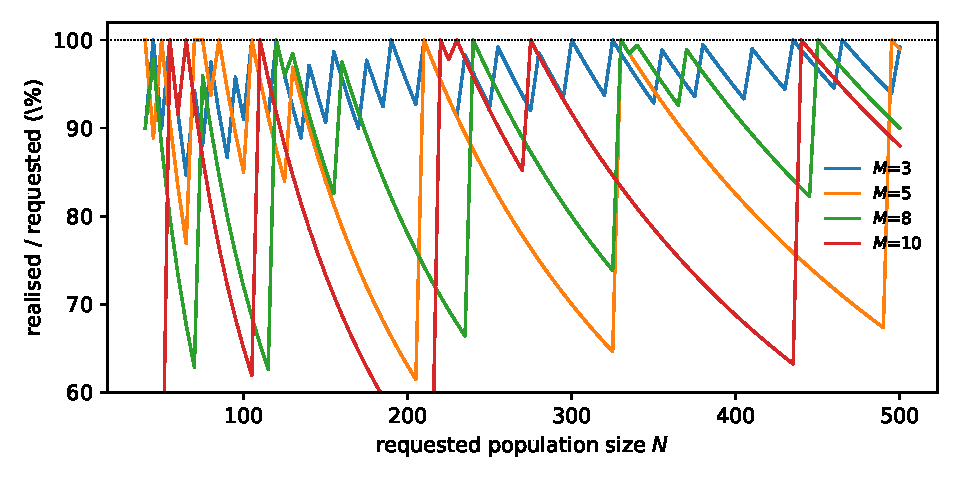
\includegraphics[width=0.63\textwidth]{fig_deficit.pdf}
\caption{Realised population size as a fraction of the requested size for the default reference-vector constructor of PlatEMO 4.16. The realised count is a step function of the request; at the sizes used in practice it lies below the request, and the deficit grows with the number of objectives}
\label{fig:deficit}
\end{figure}

\begin{table}[!t]
\centering
\footnotesize
\caption{Realised population size returned by the default reference-vector constructor for requested sizes $N$ and objective counts $M$. Entries equal to the request are set in bold. The constructor never exceeds the request and equals it only at admissible lattice sizes}
\label{tab:deficit}
\footnotesize
\begin{tabular}{lrrrrrrrrr}
\toprule
$M$ $\backslash$ $N$ & 91 & 100 & 105 & 120 & 150 & 200 & 275 & 300 & 500 \\
\midrule
2 & \textbf{91} & \textbf{100} & \textbf{105} & \textbf{120} & \textbf{150} & \textbf{200} & \textbf{275} & \textbf{300} & \textbf{500} \\
3 & \textbf{91} & 91 & \textbf{105} & \textbf{120} & 136 & 190 & 253 & \textbf{300} & 496 \\
4 & 84 & 84 & 84 & \textbf{120} & 120 & 165 & 220 & 286 & 455 \\
5 & 85 & 85 & \textbf{105} & 105 & 126 & 126 & 210 & 210 & 495 \\
6 & 77 & 77 & 77 & 112 & 147 & 182 & 273 & 273 & 462 \\
7 & \textbf{91} & 91 & 91 & 112 & 112 & 168 & 238 & 294 & 490 \\
8 & 72 & 72 & 72 & \textbf{120} & 128 & 156 & 240 & 240 & 450 \\
9 & 90 & 90 & 90 & 90 & 90 & 174 & 210 & 210 & 495 \\
10 & 65 & 65 & 65 & 110 & 110 & 110 & \textbf{275} & 275 & 440 \\
\bottomrule
\end{tabular}

\end{table}

\subsection{Census of the distribution}
We searched the released tree. The platform ships 360 algorithms and 630 problems, organised as \nAlgTotal{} algorithm directories, one per algorithm, holding \nFilesTotal{} \texttt{.m} source files; a single algorithm is split across a main file and its helper files, so the census reports both levels. Of the \nFilesTotal{} files, \nFilesAffected{} (\pctAffected\%) contain the assignment, and they belong to \nAlgAffected{} of the \nAlgTotal{} algorithm directories, that is \pctAlgAffected\% of the algorithms in the release; \nAlgSingle{} of the \nAlgAffected{} contribute one file each and one algorithm contributes two, so \nAlgSingle{} $\times\,1 + 1\times\,2 = \nFilesAffected{}$ files across \nAlgAffected{} algorithms. The affected algorithms include the canonical NSGA-III and MOEA/D implementations and their descendants, RVEA and its variants, LMOCSO, HEA and C-TAEA, and the host itself, while \nTracedCtl{} of the sixteen algorithms we traced (\ctlNames{}) are unaffected and run at the requested size, which is what makes the comparison in Table~\ref{tab:trace} a confounded one. Table~\ref{tab:census} groups the affected algorithms by family. The assignment is not a rare idiom confined to one author, which is why the framework rather than the incident is the contribution.

\begin{table}[!t]
\centering
\footnotesize
\caption{Census of the PlatEMO 4.16 algorithm tree, at both the algorithm and the file level, for the assignment \texttt{[Z,Problem.N] = UniformPoint(Problem.N,Problem.M)}. The algorithm count is the number of directories containing at least one affected file}
\label{tab:census}
\small
\begin{tabular}{lrrl}
\toprule
family & algorithms & files & examples \\
\midrule
MOEA/D family & 26 & 26 & MOEA/D, MOEA/D-DRA, MOEA/D-DE, \dots \\
NSGA-III family & 4 & 4 & NSGA-III, A-NSGA-III, DCNSGA-III, \dots \\
RVEA family & 4 & 4 & RVEA, RVEAa, RVEA-iGNG, \dots \\
Large-scale & 14 & 15 & LMOCSO, HEA, C-TAEA, FDSEA \\
Other & 35 & 35 & AdaW, ParEGO, SPEA-R, \dots \\
\midrule
total & 83 & 84 & of 360 algorithms, 1887 files \\
\bottomrule
\end{tabular}

\end{table}

\subsection{The same request in another library}
\label{sec:xplatform}
The framework claims to be portable, so we ran the audit on a second library rather than asserting that it would apply. pymoo is a widely used Python framework with a reference-direction module of its own, and it exposes the same two constructions: a Das--Dennis lattice and a factory that returns an exact number of directions. The audit's trigger, a routine that returns a reference set together with a size that is then written into a shared population-size field, is \emph{absent} there: the Das--Dennis entry point takes the partition count and derives the cardinality, and the exact-count factory is a separate call, so no user-set population size is overwritten. The audit therefore returns a negative result on pymoo \cite{25}, which is what makes it a test rather than a tautology.

The comparison in Table~\ref{tab:xplatform} is therefore not a second defect report. What is \emph{not} absent is the underlying arithmetic, and the difference between the two libraries is instructive: the table compares the realised cardinality for the same nominal request. At three objectives both libraries return 91, because the lattice is the same; at five, eight and ten objectives they diverge, by factors of \xRatioFive{}, \xRatioEight{} and 1.18. At eight objectives a study that declares $N=100$ realises \nPlatMeight{} directions in PlatEMO and \nPymoMeight{} in pymoo, a factor of \xRatioEight{}. The divergence is not a defect of either library: PlatEMO rounds down to the largest admissible lattice and then adds a second layer, while pymoo chooses the partition count whose cardinality is closest to the request and stops there. The point for the framework is that the nominal size does not determine the realised size even across two libraries that implement the same construction, let alone across algorithms within one library, and that a comparison table reporting only the nominal size is therefore unverifiable by construction.

\begin{table}[!t]
\centering
\footnotesize
\caption{Realised cardinality of the reference set for the same nominal request in two libraries. The first row gives the requested size and the second the number of objectives; the last row is the ratio of the PlatEMO value to the pymoo value. The two agree when the request happens to be an admissible single-layer lattice size and diverge otherwise}
\label{tab:xplatform}
\footnotesize
\setlength{\tabcolsep}{7pt}
\begin{tabular}{lrrrrr}
\toprule
library & $100$ & $100$ & $100$ & $100$ & $200$ \\
($N_{\mathrm{req}}$) & $3$ & $5$ & $8$ & $10$ & $3$ \\
\midrule
PlatEMO 4.16 & 91 & 85 & 72 & 65 & 190 \\
pymoo 0.6.2 & 91 & 70 & 36 & 55 & 190 \\
\addlinespace
ratio & 1.00 & 1.21 & 2.00 & 1.18 & 1.00 \\
\bottomrule
\end{tabular}

\end{table}

\section{Empirical consequences of the override}
\label{sec:exp}
\subsection{Experimental setup}
\label{sec:setup}
The host is FDSEA~\cite{26}, a recent large-scale reference-vector method that contains the assignment. Its published generation loop is governed by three constants: the number of individuals exchanged between its two subpopulations ($n_{\mathrm{ex}}$, published default 10), the hybridisation weight that mixes a genetic and a differential operator ($\gamma$, published default 0.5 under an online update rule), and the neighbourhood size of the frequency-domain subpopulation ($K$, published default 5). We hold $K$ at 5 and set the other two statically, so that the effect of the population size is separated from the effect of the constants. We compare nine configurations of the same host, all single-threaded, all with an evaluation budget of $\budget$ and seeds $1,\dots,\seeds$ for the $D=300$ problems and \seedsExt{} for the $M=5$ and $D=1000$ problems: the host as published; the host with the size output discarded (repair~1); the host with the exactly-$N$ constructor (repair~2); an adaptive scheduling layer that updates $n_{\mathrm{ex}}$, $\gamma$ and $K$ online from a convergence and a diversity signal, used later only as a case study; and five static settings of $n_{\mathrm{ex}}$ and $\gamma$. They appear, respectively, in Table~\ref{tab:abc} (published and repair~1 --- there named ``repaired'' --- alongside the declared control) and, in the supporting information, Tables~S3 (repair~2), S5 (layer), S1 (static settings) and S2 (the separate $K$ sweep). The suite has \nProbs{} problems: DTLZ1, DTLZ2 and DTLZ7~\cite{27} and the nine instances LSMOP1--LSMOP9~\cite{28} at $M=3$, $D=300$; LSMOP1 and LSMOP6 at $M=5$, $D=500$; and LSMOP1 at $M=3$, $D=1000$. The indicator is the inverted generational distance~\cite{29} to a \refFrontPts{}-point discretisation of the true front; for every front used here the front spans the unit interval in each objective, so the usual normalisation is the identity.

Two points about the design determine how the results are to be read. First, the comparison isolates something narrower than the framework as a whole. All nine configurations are launched with the same requested size $N=100$, and Section~\ref{sec:abc} adds a further declared arm to separate the two effects below; ``as published'' realises $N_{\mathrm{real}}=91$ because the override takes effect, and ``repair~1'' realises $N_{\mathrm{real}}=100$. The measured difference is therefore the difference between the declared condition and the realised one, and by construction it coincides with the difference between a 91-individual and a 100-individual run of the host. We do not claim that fidelity has an effect separable from the population size; we claim, and measure, that declaring one size while running another changes the conclusion a study would draw. Second, the termination test is evaluated at generation boundaries, so a run can overshoot the budget by less than one generation: the published arm consumes \feHost{} evaluations (\feOverPct\% above nominal) and the corrected arms \feFix{} exactly.

Algorithms share seeds, so the runs are paired and we use the two-sided Wilcoxon signed-rank test, reporting also the Holm--Bonferroni correction over the \nProbs{} comparisons, the sign test, and Cliff's delta as an effect size that does not assume a distribution. Throughout, the central tendency is reported as the \emph{median} over the runs, the interquartile range of the per-run record is used as spread, and every percentage change quoted in the text, in the tables and in Figure~\ref{fig:main} is computed from medians as a ratio of medians, so that the three agree; optimisation runs occasionally produce a few dominating outliers, and the median is the robust summary. The raw per-run records are released, so the mean can be recovered exactly.

\subsection{Three arms: declared, realised and repaired}
\label{sec:abc}
Because the published configuration differs from the repaired one in the population actually evaluated, a comparison between those two alone cannot say whether the problem is the declaration or the size. We therefore ran a third arm in which the host is configured at the size it will realise --- \retMthree{} at three objectives and \retMfive{} at five, which are the two values the constructor returns for a request of 100 at those objective counts (Table~\ref{tab:deficit}) --- so that the declaration and the realisation agree. The three arms are then \emph{published} (declared 100, realised \retMthree{}), \emph{declared} (declared \retMthree{}, realised \retMthree{}) and \emph{repaired} (declared 100, realised 100). Table~\ref{tab:abc} gives all three pairwise comparisons, and each isolates a different thing: declared against published holds the realised size fixed at \retMthree{} and varies only the declaration, so it measures the \emph{declaration} effect; repaired against declared varies the realised size from \retMthree{} to 100 at a fixed declaration, so it measures the \emph{size} effect; and repaired against published is their combination, which is the quantity a reader of the published paper actually experiences.

The declared arm requests \abcDeclReqMthree{} at three objectives and \abcDeclReqMfive{} at five, which are the values the published arm realises; the two runs therefore evaluate the same number of individuals. Their \emph{signed} median change is \abcDeclVsPubSignedMed\%, the median of the absolute changes is \abcDeclVsPubAbsMed\% and the largest is \abcDeclVsPubMax\%, and the paired signed-rank test separates none of the \nProbs{} problems: the smallest of the \abcPairs{} p-values is \abcMinP{} (Table~S6 lists them). This is the direct evidence for the motivating claim: a run that declares 100 and a run that declares \retMthree{} are the same run, because both evaluate \retMthree{} individuals; whatever a study reports, the population it used is the one the constructor returned. The residual differences are of the order of one per cent and change sign across problems, as expected when the only difference is that the two arms initialise different numbers of candidates before the first selection. Against that, repaired and declared differ by a median of \abcRepVsDeclMed\%, which is the pure realised-size effect. Read against the published arm instead, the repaired host is better on \abcRepVsPubPos{} problems, identical on \abcRepVsPubTie{} and worse on \abcRepVsPubNeg{}, with a median of \abcRepVsPubMed\%; that is the count the abstract reports. The three arms therefore separate the two effects the single comparison conflates, and they locate the defect where the framework puts it: not in the algorithm, which behaves as the realised size dictates, but in the number printed beside the result.

\begin{table}[!t]
\centering
\footnotesize
\caption{Three-arm comparison: published, declared and repaired, on the same host and seeds. Published declares 100 and realises \retMthree{}; declared declares and realises \retMthree{} (the request is \abcDeclReqMthree{} at three objectives and \abcDeclReqMfive{} at five); repaired declares and realises 100. The three right-hand columns are median relative changes of the first-named arm against the second, positive meaning the first attains a smaller indicator, so that \emph{decl\,$-$\,pub} isolates the declaration effect at a fixed realised size, \emph{rep\,$-$\,decl} the realised-size effect at a fixed declaration, and \emph{rep\,$-$\,pub} their combination}
\label{tab:abc}
\footnotesize
\setlength{\tabcolsep}{4pt}
\begin{tabular}{lccc rr}
\toprule
problem & published & declared & repaired & declared$-$pub & repaired$-$dec \\
\midrule
DTLZ1 & 0.0657 & 0.0670 & 0.0584 & $-1.9\%$ & $+12.8\%$ \\
DTLZ2 & 0.0609 & 0.0620 & 0.0603 & $-1.8\%$ & $+2.7\%$ \\
DTLZ7 & 0.0590 & 0.0598 & 0.0543 & $-1.3\%$ & $+9.1\%$ \\
LSMOP1 & 0.1032 & 0.1035 & 0.0945 & $-0.3\%$ & $+8.7\%$ \\
LSMOP2 & 0.0812 & 0.0807 & 0.0823 & $+0.5\%$ & $-2.0\%$ \\
LSMOP3 & 0.8645 & 0.8645 & 0.8645 & $+0.0\%$ & $+0.0\%$ \\
LSMOP4 & 0.1448 & 0.1408 & 0.1424 & $+2.8\%$ & $-1.2\%$ \\
LSMOP5 & 0.3559 & 0.3554 & 0.3531 & $+0.1\%$ & $+0.7\%$ \\
LSMOP6 & 0.6429 & 0.6428 & 0.6363 & $+0.0\%$ & $+1.0\%$ \\
LSMOP7 & 0.8052 & 0.8052 & 0.8383 & $+0.0\%$ & $-4.1\%$ \\
LSMOP8 & 0.0769 & 0.0778 & 0.0748 & $-1.2\%$ & $+3.9\%$ \\
LSMOP9 & 0.7359 & 0.7358 & 0.7351 & $+0.0\%$ & $+0.1\%$ \\
LSMOP1 (5,500) & 0.3971 & 0.3904 & 0.3736 & $+1.7\%$ & $+4.3\%$ \\
LSMOP6 (5,500) & 0.9400 & 0.9001 & 0.8693 & $+4.2\%$ & $+3.4\%$ \\
LSMOP1 (3,1000) & 0.0992 & 0.1013 & 0.0904 & $-2.2\%$ & $+10.8\%$ \\
\bottomrule
\end{tabular}

\end{table}

\subsection{Effect of restoring fidelity on the host}
\label{sec:effect}
Table~\ref{tab:abc} reports the host on all \nProbs{} problems, Table~S3 of the supporting information adds repair~2, and Figure~\ref{fig:main} shows the per-problem median change. Restoring the requested size changes the median indicator from \fixMinGain\% to \fixMaxGain\%, the median change over the suite being \fixMedGain\%. The direction of the effect is not uniform, and we state the counts exactly rather than in summary. These counts are against the published arm --- the \emph{rep\,$-$\,pub} column of Table~\ref{tab:abc} --- which measures the combined declaration-and-size effect; the pure realised-size effect (\emph{rep\,$-$\,decl}) is reported in Section~\ref{sec:abc}. The corrected host is no worse on \fixNoWorseN{} of the \nProbs{} problems and worse on the remaining \fixWorseN{}. We give the breakdown rather than a single count: twelve of the \fixNoWorseN{} improve clearly, LSMOP3 is a tie (the medians differ by about $3\times10^{-6}$, so the printed value is $+0.0\%$), and the two degradations are LSMOP2 and LSMOP7, both by a small margin. The pure size effect (\emph{rep\,$-$\,decl} in Table~\ref{tab:abc}) degrades three problems: LSMOP2, LSMOP4 and LSMOP7; LSMOP4 appears neutral in the combined count because the declaration effect offsets its size effect. This is Proposition~2's fixed-budget trade-off in miniature: the extra nine individuals buy wider coverage and cost about a tenth of the generations, and on those three problems the lost generations outweigh the added coverage. Read as \emph{no worse}, the count is thirteen; read as \emph{improved}, it is twelve, and we use the latter in the abstract.

Statistical significance is weaker than the direction count. The change is significant on \fixSigCount{} of the \nProbs{} problems at the uncorrected $0.05$ level, and on \fixSigHolm{} problem after Holm--Bonferroni correction; the single survivor is an $M=5$ instance, where the realised deficit is largest. Power over fifteen comparisons is limited at thirty seeds, so we complement the tests with an effect size that does not depend on a distributional assumption: Cliff's delta ranges in magnitude up to \cliffMax{}. Independently, a bootstrap confidence interval for the median difference excludes zero on \ciExclN{} of the \nProbs{} problems. That count is larger than the corrected test because the interval is not adjusted for multiplicity, so we report it as exploratory and lead with the corrected count rather than with the interval. The honest reading: the direction of the effect is consistent across the suite, its magnitude is confidently non-zero on about half the problems, and Proposition~1 bounds the sign rather than the size.

Two points deserve emphasis. First, the effect is an improvement and not a neutral re-ranking: the override under-estimates what the host achieves at its reported size, so a study that prints $N=100$ and runs \retMthree{} individuals publishes a number that belongs to a smaller configuration. Second, the direction of the mean can disagree with the median and with the majority of runs when a few outliers dominate: on DTLZ7 the corrected host is better on \dtlzSevenWins{} of the \seeds{} runs and by median, yet its mean is worse --- which is why a single mean hides the effect.

\begin{figure}[!t]
\centering
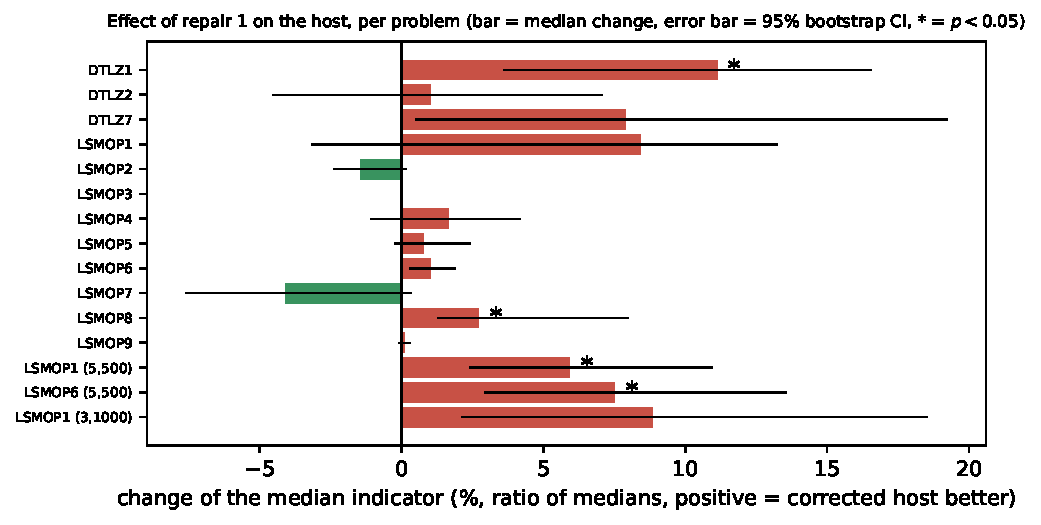
\includegraphics[width=0.78\textwidth]{fig_main.pdf}
\caption{Change of the median indicator of the host from restoring the requested population size, shown separately for each of the fifteen problems; the bar is the ratio of medians, the same quantity as the repaired column of Table~\ref{tab:abc}, the error bar is a bootstrap 95\% confidence interval for the median difference, and an asterisk marks $p<0.05$ before correction}
\label{fig:main}
\end{figure}

\begin{table}[!t]
\centering
\footnotesize
\caption{Wilcoxon signed-rank test of repair 1 against the published host. The baseline is the published run, which Section~\ref{sec:abc} shows is statistically the same as the declared arm (the paired signed-rank test separates none of the \nProbs{} problems; Table~S6), so this table measures the combined declaration-and-size effect; Section~\ref{sec:abc} separates the two. ``Repair 1 wins'' counts the runs on which the corrected host attains a smaller indicator}
\label{tab:sig}
\footnotesize
\setlength{\tabcolsep}{5pt}
\begin{tabular}{lrrrrr}
\toprule
problem & repair 1 wins & $p$ (signed rank) & Holm--Bonferroni & sign test & Cliff $\delta$ \\
\midrule
DTLZ1 & 21/30 & 0.0155 & 0.1855 & 0.0428 & +0.45 \\
DTLZ2 & 18/30 & 0.3387 & 1.0000 & 0.3616 & +0.14 \\
DTLZ7 & 20/30 & 0.0879 & 0.7914 & 0.0987 & +0.32 \\
LSMOP1 & 18/30 & 0.0549 & 0.6041 & 0.3616 & +0.33 \\
LSMOP2 & 12/30 & 0.1840 & 1.0000 & 0.3616 & -0.20 \\
LSMOP3 & 14/30 & 0.7151 & 1.0000 & 0.8555 & -0.02 \\
LSMOP4 & 15/30 & 0.4522 & 1.0000 & 1.0000 & +0.15 \\
LSMOP5 & 19/30 & 0.4400 & 1.0000 & 0.2005 & +0.23 \\
LSMOP6 & 19/30 & 0.0699 & 0.6989 & 0.2005 & +0.37 \\
LSMOP7 & 15/30 & 0.3931 & 1.0000 & 1.0000 & -0.23 \\
LSMOP8 & 22/30 & 0.0099 & 0.1291 & 0.0161 & +0.45 \\
LSMOP9 & 17/30 & 0.8078 & 1.0000 & 0.5847 & +0.13 \\
LSMOP1 (5,500) & 19/20 & $<10^{-4}$ & $2.9e-04$ & $<10^{-4}$ & +0.59 \\
LSMOP6 (5,500) & 17/20 & 0.0037 & 0.0512 & 0.0026 & +0.64 \\
LSMOP1 (3,1000) & 14/20 & 0.0973 & 0.7914 & 0.1153 & +0.44 \\
\bottomrule
\end{tabular}

\end{table}

\subsection{Two ways of restoring fidelity}
\label{sec:repairs}
Section~\ref{sec:abc} used the conservative repair to separate declaration from size; this subsection asks which of the two admissible repairs to prefer, because they change different things. Table~S3 of the supporting information gives repair~2 alongside repair~1. The two repairs are not equivalent: repair~2 changes the reference set as well as the population --- a comparison against repair~1 measures two things at once --- and on several problems the default constructor's smaller reference set is at least as good. Where the algorithm permits the population to differ from the reference set, repair~1 is the conservative choice, because it changes exactly one thing; which repair is admissible depends on the algorithm, as Section~\ref{sec:across} shows.

\subsection{A reported gain undone by the override}
\label{sec:case-layer}
To show how the override manufactures a gain we use the adaptive scheduling layer that originally motivated this work; it drives $n_{\mathrm{ex}}$, $\gamma$ and $K$ online from a convergence and a diversity signal. It is a case study, not a contribution, reported on all \nProbs{} problems (Table~S5). Against the published host the layer is better on \layerBetterHost{} problems and worse on the other \layerWorseHost{}, with a median gain of only \layerMedHost\%: the double-digit gains that motivated it are concentrated in \layerBigN{} problems and absent elsewhere. Against the host at the requested population size, which isolates the scheduling, the picture narrows further: better on \layerBetterMatched{} problems, worse on \layerWorseMatched{}, median \layerMedMatched\%. Six of the fifteen, chosen to span the three regimes (first figure against the published host, second against the matched one; Table~S5 lists all fifteen), are: a gain that survives matching --- DTLZ1 ($+36.0\%$, $+28.0\%$), DTLZ2 ($+13.3\%$, $+12.4\%$) and LSMOP1 ($+15.5\%$, $+7.7\%$); a gain that halves --- DTLZ7 ($+14.2\%$, $+6.8\%$); and problems where the layer loses outright --- LSMOP2 ($-6.3\%$, $-4.7\%$) and LSMOP6 ($-2.2\%$, $-3.3\%$). On the \layerBigN{} problems carrying a gain above 5\%, matching the size removes \layerShrinkMin{} to \layerShrinkMax{} percentage points of it, so much of the apparent advantage is the population difference rather than the scheduling; the remaining nine stay within \layerSmallMax\% in either direction, and their signs split four in the layer's favour and five against. The layer and the static settings of Section~\ref{sec:static} both run at the requested population size: against the best static setting the layer attains a smaller median on only \layerBeatsStaticN{} of the \nProbs{} problems, including \layerStrongBeatsN{} of the \layerStrongN{} where its gain over the published host exceeds 5\%. We therefore do not claim that the layer is worthless; we claim that the evidence which previously supported it was largely an artefact of comparing a 100-individual layer against a 91-individual host, and that at a matched size the advantage is small and inconsistent in sign.

\subsection{Consequence across algorithms}
\label{sec:across}
The affected set is not confined to one family. A comparison table that mixes affected and unaffected methods is therefore confounded, because the affected methods run with fewer individuals than they report. Table~\ref{tab:peer} quantifies this on NSGA-III. The picture is more equivocal than for the host: the corrected NSGA-III is better on LSMOP1 but worse on LSMOP4 and LSMOP6, and the signed-rank test is significant on LSMOP2 and LSMOP4 even where the medians barely move, because the override also changes the shape of the run-to-run distribution rather than only its centre. There is accordingly no uniform sign to the bias.

We attempted the same repair on the other affected peers, where the catalogue of Section~\ref{sec:catalogue} becomes concrete. NSGA-III is case~A and accepts repair~1. MOEA/D is case~B: it indexes its individuals by reference vector, and repair~1 fails with an index-out-of-bounds error, while repair~2 restores it. RVEA and LMOCSO~\cite{30} are case~C: both compute the smallest inter-vector angle $\gamma_i=\min_j\arccos(1-\mathrm{d}_{\cos}(v_i,v_j))$, with $\mathrm{d}_{\cos}$ the cosine distance, and divide the convergence term by $\gamma_i$. The mechanism is the one measured in Table~\ref{tab:angle}: the exactly-$N$ constructor reduces the smallest angle by a factor of \angRatioThree{} at $M=3$ and \angRatioFive{} at $M=5$, so $\gamma_i$ falls and the convergence term is amplified in proportion --- a quantitative degradation, and the reason the case needs its own repair. Repair~1 fails for RVEA as well, though later than MOEA/D's immediate failure: RVEA runs until the first reference-vector adaptation, which the platform schedules at $f_r = 0.1$ of the planned generations, where the assignment $V(1:N,:)$ requires the vector set to have at least $N$ rows. Table~S7 of the supporting information reports the catalogue validation on DTLZ1--7 at three objectives (PlatEMO's DTLZ defaults: dimension $M{+}4$ for DTLZ1, $M{+}9$ for DTLZ2--6 and $M{+}19$ for DTLZ7; requested $N{=}100$; the budget of Section~\ref{sec:exp}). Repair~2 restores MOEA/D, which runs at exactly 100 individuals throughout: on DTLZ1--4 its median IGD stays within 3\% (relative) of the published arm and on DTLZ5--7 it improves (0.016, 0.016 and 0.091 against 0.040, 0.040 and 0.102); every one of those seven differences is significant in a paired signed-rank test (uncorrected $p \le 0.033$; all seven survive Holm correction).

On the degenerate fronts the unbounded constructor degrades the Case~C pairs: RVEA's median IGD on DTLZ5 and DTLZ6 rises from 0.074 and 0.139 to 0.232 and 0.340, and LMOCSO's on DTLZ5 and DTLZ6 from 0.039 and 0.040 to 0.920 and 0.958; the bounded-angle constructor repairs that damage, giving RVEA 0.039 on DTLZ1 and 0.061 and 0.097 on DTLZ5 and DTLZ6 --- better than its published arm on all seven problems (Table~S7) --- and LMOCSO to 0.040 on both, the two values coinciding to three digits. The bounded-angle repair is validated on the DTLZ family; its behaviour on the large-scale LSMOP suite is left to the released scripts and to future work.

Fidelity can accordingly be restored everywhere but not uniformly: the admissible repair follows from the coupling between population and reference set, not from a universal rule.

\begin{table}[!t]
\centering
\footnotesize
\caption{NSGA-III with the published override and with the requested population size restored by repair 1, on six large-scale problems. NSGA-III is case~A, so repair~1 leaves the reference set untouched; the realised population is \retMthree{} in the published row and 100 after the repair, as in Table~\ref{tab:abc}}
\label{tab:peer}
\resizebox{\textwidth}{!}{
\footnotesize
\setlength{\tabcolsep}{4pt}
\begin{tabular}{lcccccc}
\toprule
NSGA-III (median) & LSMOP1 & LSMOP2 & LSMOP4 & LSMOP6 & LSMOP8 & LSMOP9 \\
\midrule
as published & 0.6288 & 0.0829 & 0.1963 & 2.9299 & 0.3459 & 1.0834 \\\\
repair 1 (requested $N$) & 0.5832 & 0.0836 & 0.1999 & 3.5033 & 0.3437 & 1.0770 \\\\
\addlinespace
$p$ (signed rank) & 0.0841 & 0.0155 & $6.7e-04$ & 0.5291 & 0.9354 & 0.0767 \\\\
\bottomrule
\end{tabular}
}

\end{table}

\subsection{Static settings and cost}
\label{sec:static}
Sweeping the two constants statically (Table~S1 of the supporting information) suggests that the exchange count is the load-bearing one, and it provides the reference against which the layer of Section~\ref{sec:case-layer} is judged; it is context for the case study only, and therefore lives in the supporting information. The host as published completes \genHost{} generations and the corrected host \genFix{}, a ratio of \genRatio{} against the ratio of realised population sizes, \popRatio{}, as Proposition~2 predicts. The small excess over the predicted ratio comes from the evaluation accounting rather than from the population: the host keeps two subpopulations and consumes about $2N$ evaluations per generation, so one generation of the published arm costs fewer evaluations than one generation of the corrected arm, and the generation-boundary termination test lets the published run stop \feOver{} evaluations (\feOverPct\%) past the nominal budget. The wall-clock differences follow from the same effect and are not evidence about the algorithm.

The same static family checks that the comparison between the layer and the static settings of Section~\ref{sec:case-layer} is made over the same search space: the layer updates $K$ online, the static settings held it at its published value; Table~S2 of the supporting information closes that gap by sweeping $K \in \{3,5,10\}$ at a fixed exchange count and hybridisation weight. The sensitivity is not marginal. The best value differs across problems (\kWinsThree{} problems prefer $K{=}3$, \kWinsFive{} prefer $K{=}5$ and \kWinsTen{} prefer $K{=}10$), with a median spread of \kSpreadMed\% of the indicator between the best and the worst of the three settings. A median spread understates the case: on \kFailProblem{}, $K{=}\kFailK{}$ yields a median indicator of \kFailValue{} against \kFailBest{} for $K{=}3$, a factor of \kFailRatio{}, and the failure is not one unlucky seed, since \kFailBadSeeds{} of the \seeds{} runs at that setting exceed unity. The evaluation counts match the budget --- Table~\ref{tab:cost} and its note cover the $K$ sweep, recorded at exactly the nominal $\budget$ per run --- so the runs completed; those runs simply do not converge, and on \kFailN{} of the \nProbs{} problems the choice of $K$ changes the outcome by more than an order of magnitude. This matters for the case study, because the adaptive layer updates $K$ online over a range that contains the failing value: a static choice of $K$ cannot be treated as neutral in either direction.

\begin{table}[!t]
\centering
\footnotesize
\caption{Population, evaluations, generations and wall-clock time; the $K$ sweep (Table~S2) is recorded at exactly $\budget$ evaluations per run}
\label{tab:cost}
\footnotesize
\setlength{\tabcolsep}{7pt}
\begin{tabular}{lrrrr}
\toprule
configuration & population & evaluations & generations & wall (s) \\
\midrule
as published & 91 & 100090 & 552 & 18.9 \\
requested $N$ & 100 & 100000 & 499 & 18.5 \\
\bottomrule
\end{tabular}

\end{table}

\section{Discussion and conclusion}
\label{sec:conclusion}
We have argued that the population size of a reference-vector MOEA is a controlled quantity that can silently stop being controlled, and we have given a framework that makes the failure detectable, repairable and reportable. Applied to PlatEMO 4.16, the framework reveals that \nFilesAffected{} of \nFilesTotal{} algorithm source files, belonging to \nAlgAffected{} of \nAlgTotal{} algorithms, overwrite the requested population size with the size of an approximate reference lattice that never exceeds the request and is exact in only \retExactFrac\% of cases; at the sizes in common use the reduction reaches \retWorst\%. On a large-scale suite, restoring the requested size leaves the host's median indicator no worse on thirteen of fifteen problems (twelve clear improvements and one tie, LSMOP3) and worse on two (LSMOP2 and LSMOP7); significance is limited --- four at the uncorrected $0.05$ level, one after Holm--Bonferroni --- and an exploratory, uncorrected bootstrap interval excludes zero on \ciExclN{} of the \nProbs{} problems; it accounts for most of the median scheduling gain that had been attributed to the scheduler, leaving a small and sign-inconsistent remainder; and it changes sign across peers, so that no single repair is universally admissible.

Two conclusions follow, and they are methodological rather than algorithmic. The first is that the framework converts a diffuse worry about experimental fairness into a procedure with four checkable outputs: an audit that yields a census at the algorithm and file level, a deficit table, a repair catalogue with the mechanism of the hardest case measured, and a reporting protocol. Any library that returns a reference set together with a size can be audited in the same way, and any of the three repair cases can be recognised from the coupling between population and reference set rather than by trial and error. The second is that the finding should be read as a reporting concern and not as a defect in the algorithms: the rounding performed by a simplex lattice is unavoidable, the write-back is often deliberate, and no run in this study is in any way broken. What is avoidable is publishing a table that states a size the run did not use, which is the one thing the framework asks a study not to do. The recent finding that thirteen widely used frameworks differ in ways that change comparison outcomes, even at identical settings, indicates that the audit is worth running more broadly~\cite{10}.

The framework is deliberately stated so that it does not depend on PlatEMO. The trigger it looks for is a constructor that returns a reference set together with a size which is then written into a shared population-size field, and this pattern is not specific to one library: it appears wherever a convenience routine both samples reference vectors and reports how many it sampled. The audit of Algorithm~1 can therefore be applied unchanged to any such library, and the deficit function $\delta$ can be tabulated once per constructor. The three repair cases are likewise recognised from the coupling between population and reference set rather than from the identity of the algorithm, so a practitioner who can answer the single question ``must the population equal the reference set?'' can select the admissible repair.

The study has clear limits. The audit covers one distribution at one version, so the census measures PlatEMO 4.16 and is not a survey; extending it is the necessary next step before the pattern's portability can be asserted rather than argued. The empirical magnitude is host- and suite-dependent, and the comparison between the declared and the realised configuration coincides by construction with a difference in population size, so we quantify a reporting error rather than an intrinsic property of fidelity. The $M=5$ and $D=1000$ parts of the suite are smaller than the $D=300$ part, and thirty seeds give limited power over fifteen simultaneous comparisons, which is why we report effect sizes alongside tests. The case-study layer is one design; we do not claim that no scheduler of this family could add value, only that the evidence for this one was confounded and that at a matched size it is small. Finally, the framework detects and repairs infidelity but cannot decide how large a population should be --- a modelling choice for the practitioner.

\noindent\textbf{Data availability.} The release is publicly available at \url{github.com/qingdi-miruisi/population-size-fidelity}, at tag v1.17, which pins one immutable commit, and contains the audit script of Algorithm~1, the per-file audit listing, the realised-count table $L(N,M)$ over \retCombos{} combinations, the trace and cross-library tables, the corrected variants for the three repair cases, the driver scripts that regenerate every table and figure, and the raw per-run archives from which all reported statistics are recomputed. No file of the audited distribution was modified; all experiments ran in MATLAB R2026a against PlatEMO 4.16 with the recorded seeds and are single-threaded.

\noindent\textbf{Conflict of interest.} The author declares that he has no conflict of interest: the audited platform is an open-source community project with which he has no financial or personal relationship.

\noindent\textbf{Author contributions.} The sole author, Y. X. Zhang, was responsible for all aspects of the work.

%%%%%%%%%%%%%%%%%%%%%%%%%%%%%%%%%%%%%%%%%%%%%%%%%%%%%%%
%%% Acknowledgements
%%%%%%%%%%%%%%%%%%%%%%%%%%%%%%%%%%%%%%%%%%%%%%%%%%%%%%%
\Acknowledgements{This research received no external funding. The author thanks the developers of PlatEMO for making the platform and its source code openly available, which is what makes an audit of this kind possible.}

%%%%%%%%%%%%%%%%%%%%%%%%%%%%%%%%%%%%%%%%%%%%%%%%%%%%%%%
%%% Supplements
%%%%%%%%%%%%%%%%%%%%%%%%%%%%%%%%%%%%%%%%%%%%%%%%%%%%%%%
\Supplements{Tables S1--S7: static settings; $K$ sensitivity; repair~2 alongside repair~1; the bounded-angle constructor; the scheduling layer against both references; p-values; the catalogue validation on DTLZ1--7. Also the parser test suite, the per-file audit listing, the realised-count table, the measured angles, the corrected variants and the raw per-run records.}

%%%%%%%%%%%%%%%%%%%%%%%%%%%%%%%%%%%%%%%%%%%%%%%%%%%%%%%
%%% References
%%%%%%%%%%%%%%%%%%%%%%%%%%%%%%%%%%%%%%%%%%%%%%%%%%%%%%%
\begin{thebibliography}{99}
\bibitem{1} Deb K, Jain H. An evolutionary many-objective optimization algorithm using reference-point-based nondominated sorting approach, part I: solving problems with box constraints. IEEE Trans Evol Comput, 2014, 18: 577--601
\bibitem{2} Zhang Q, Li H. MOEA/D: a multiobjective evolutionary algorithm based on decomposition. IEEE Trans Evol Comput, 2007, 11: 712--731
\bibitem{3} Cheng R, Jin Y, Olhofer M, et al. A reference vector guided evolutionary algorithm for many-objective optimization. IEEE Trans Evol Comput, 2016, 20: 773--791
\bibitem{4} Wu X, Wu S H, Wu J, et al. Evolutionary computation in the era of large language model: survey and roadmap. IEEE Trans Evol Comput, 2024, 29: 177--208
\bibitem{5} Liu F, Lin X, Yao S, et al. Large language model for multiobjective evolutionary optimization. In: Proceedings of the International Conference on Evolutionary Multi-Criterion Optimization, Singapore, 2025. 178--191
\bibitem{6} Huang Y, Wu S, Zhang W, et al. Autonomous multi-objective optimization using large language model. IEEE Trans Evol Comput, 2025, in press
\bibitem{7} Liu J, Sarker R, Elsayed S, et al. Large-scale evolutionary optimization: a review and comparative study. Swarm Evol Comput, 2024, 85: 101466
\bibitem{8} Wang P, Wu X, Deng H. Large-scale multi-objective optimization algorithms: a decade survey. Expert Syst, 2025, 42: e70157
\bibitem{9} Ishibuchi H, Pang L M, Shang K. Population size specification for fair comparison of multi-objective evolutionary algorithms. In: Proceedings of the IEEE International Conference on Systems, Man, and Cybernetics, Toronto, 2020. 1095--1102
\bibitem{10} Ravber M, Smid M, Moravec M, et al. Performance comparison of single-objective evolutionary algorithms implemented in different frameworks. Informatica, 2025, 36: 677--712
\bibitem{11} Tian Y, Cheng R, Zhang X, et al. PlatEMO: a MATLAB platform for evolutionary multi-objective optimization. IEEE Comput Intell Mag, 2017, 12: 73--87
\bibitem{12} Lopez-Ibanez M, Branke J, Paquete L. Reproducibility in evolutionary computation. ACM Trans Evol Learn Optim, 2021, 1: 14:1--14:21
\bibitem{13} Yang L, Zhang Y, Cao J, et al. A many-objective evolutionary algorithm based on reference vector guided selection and two diversity and convergence enhancement strategies. Appl Soft Comput, 2024, 154: 111369
\bibitem{14} Derrac J, Garcia S, Molina D, et al. A practical tutorial on the use of nonparametric statistical tests as a methodology for comparing evolutionary and swarm intelligence algorithms. Swarm Evol Comput, 2011, 1: 3--18
\bibitem{15} Demsar J. Statistical comparisons of classifiers over multiple data sets. J Mach Learn Res, 2006, 7: 1--30
\bibitem{16} Lian J J. Time-fair benchmarking for metaheuristics: a restart-fair protocol for fixed-time comparisons. arXiv:2509.08986, 2025
\bibitem{17} Molina D, Del Ser J, Poyatos J, et al. The paradox of success in evolutionary and bioinspired optimization: revisiting critical issues, key studies, and methodological pathways. Swarm Evol Comput, 2025, 98: 102063
\bibitem{18} Kononova A V, van Stein N, Mersmann O, et al. Benchmarking that matters: rethinking benchmarking for practical impact. arXiv:2511.12264, 2025
\bibitem{19} Yao S, Liu F, Lin X, et al. Multi-objective evolution of heuristic using large language model. In: Proceedings of the AAAI Conference on Artificial Intelligence, Philadelphia, 2025. 27144--27152
\bibitem{20} Zhou M C, Cui M, Xu D, et al. Evolutionary optimization methods for high-dimensional expensive problems: a survey. IEEE/CAA J Autom Sinica, 2024, 11: 1092--1105
\bibitem{21} Liang J, Lou Y, Yu M, et al. A survey of surrogate-assisted evolutionary algorithms for expensive optimization. J Membr Comput, 2025, 7: 108--127
\bibitem{22} Liu Z, Han F, Ling Q, et al. Constraint-Pareto dominance and diversity enhancement strategy-based evolutionary algorithm for solving constrained multiobjective optimization problems. IEEE Trans Evol Comput, 2025, 29: 2771--2784
\bibitem{23} Tian Y, Xiang X, Zhang X, et al. Sampling reference points on the Pareto fronts of benchmark multi-objective optimization problems. In: Proceedings of the IEEE Congress on Evolutionary Computation, Rio de Janeiro, 2018. 1--6
\bibitem{24} Das I, Dennis J E. Normal-boundary intersection: a new method for generating the Pareto surface in nonlinear multicriteria optimization problems. SIAM J Optim, 1998, 8: 631--657
\bibitem{25} Blank J, Deb K. Pymoo: multi-objective optimization in Python. IEEE Access, 2020, 8: 89497--89509
\bibitem{26} Wang W, Tan Z, Wang Y, et al. Enhancing the scalability of large-scale multi-objective evolutionary algorithm through frequency domain search. Swarm Evol Comput, 2026, 106: 102423
\bibitem{27} Deb K, Thiele L, Laumanns M, et al. Scalable multi-objective optimization test problems. In: Proceedings of the IEEE Congress on Evolutionary Computation, Honolulu, 2002. 825--830
\bibitem{28} Cheng R, Jin Y, Olhofer M. Test problems for large-scale multiobjective and many-objective optimization. IEEE Trans Cybern, 2017, 47: 4108--4121
\bibitem{29} Zitzler E, Thiele L. Multiobjective evolutionary algorithms: a comparative case study and the strength Pareto approach. IEEE Trans Evol Comput, 1999, 3: 257--271
\bibitem{30} Tian Y, Zheng X, Zhang X, et al. Efficient large-scale multi-objective optimization based on a competitive swarm optimizer. IEEE Trans Cybern, 2020, 50: 3696--3708

\end{thebibliography}

\end{document}
